\section{Технологический раздел}

\subsection{Средства реализации системы}

\subsubsection{Выбор СУБД}

В качестве наиболее подходящей системы управления базами данных выбрана система PostgreSQL~\cite{postgres}~--~объектно-реляционная СУБД с открытым кодом. 
Выбор основан на исследованиях~\cite{taipalus-DBMS-survey}, которые утверждают, что самыми быстрыми по операции чтения реляционными СУБД являются MySQL~\cite{mysql}, PostgreSQL и SQL Server~\cite{sql-server}. 
При этом SQL Server, в отличие от MySQL и PostgreSQL является коммерческой СУБД, что является препятствием для её использования в данном проекте. 
Что касается MySQL, то в данной СУБД отсутствует возможность создания табличных функций~\cite{mysql-functions}, что не позволит реализовать спроектированные алгоритмы.

Что касается кеширующей базы данных, выбор пал на In-Memory Database (IMDB) Redis~\cite{redis}. Согласно тем же исследованиям~\cite{taipalus-DBMS-survey}, она является одной и самых быстрых NoSQL СУБД, и, поскольку не предъявляются требования к наличию хранимых процедур для кеширующей базы данных, Redis предоставляет весь необходимый функционал.

\subsubsection{Выбор языка программирования}

Во многих современных языках программирования реализованы библиотеки для работы с PostgreSQL. 
Не исключением является и язык C$\#$~\cite{c-sharp}, выбранный в качестве основного языка программирования в данном проекте. 
Данный выбор связан с тем, что C$\#$ -- один из наиболее активно развивающихся~\cite{tiobe} кросс-платформенных языков программирования с открытым исходным кодом. Множество фреймворков и библиотек на платформе .NET позволяют решить практически любую задачу.

Однако для решения поставленной задачи требуются средства обработки естественного языка. 
Язык C$\#$ не обладает достаточным набором средств NLP. 
Таким образом, часть функций необходимо реализовать на другом языке программирования. 
Для данных целей наиболее удачно подходит язык Python~\cite{python}, библиотеки для которого предоставляют огромные возможности для анализа данных -- в том числе, и лингвистических.

\subsubsection{Выбор средств разработки}

В качестве основной среды разработки выбрана среда JetBrains Rider\\ 2022.3.2~\cite{rider}, поскольку она предоставляет обширный набор возможностей по написанию, тестированию и отладке приложений на языке C$\#$, а также встроенные статические и динамические анализаторы и отдельное окно для подключения к базам данных. 
Дополнительным преимуществом является то, что данная среда является бесплатной для студентов.

Для разработки компонента обработки лингвистических данных была выбрана среда JetBrains PyCharm 2023.1~\cite{pycharm}. 
Как и Rider, PyCharm является бесплатной для студентов и предоставляет полный набор инструментов для разработки приложений на языке Python.


\subsection{Реализация базы данных}

Для инициализации базы данных написаны SQL-сценарии, выполняющиеся при старте СУБД. 
Сценарий создания таблиц представлен в листинге~\ref{lst:create}.

Ограничения на значения столбцов таблиц представлены в листинге~\ref{lst:alter}.

Разработанная хранимая функция basic\_search представлена в листинге~\ref{lst:func}. 
Остальные разработанные функции можно найти в приложении А.

Таблицы country и language изначально заполнятся данными из файлов Countries.csv и Languages.csv. Сценарий заполнения этих таблиц представлен в листинге~\ref{lst:input}.

Реализованная ролевая модель представлена в листинге~\ref{lst:roles}.

\subsection{Реализация интерфейса для взаимодействия с базой данных}

Интерфейс доступа к базе данных реализован в виде Web API -- набора конечных точек соединения на базе фреймворка ASP.NET Core~\cite{aspnet}. 
Для удобства взаимодействия с сервером написана Swagger~\cite{swagger} документация на все контроллеры и модели системы. На основе написанной документации доступен Swagger UI, позволяющий интерактивно взаимодействовать с API. 
Начальная страница Swagger UI разработанного приложения представлена на рисунке~\ref{swagger}.

\captionsetup{singlelinecheck = false, justification=centering}
\begin{figure}[H]
	\centering
	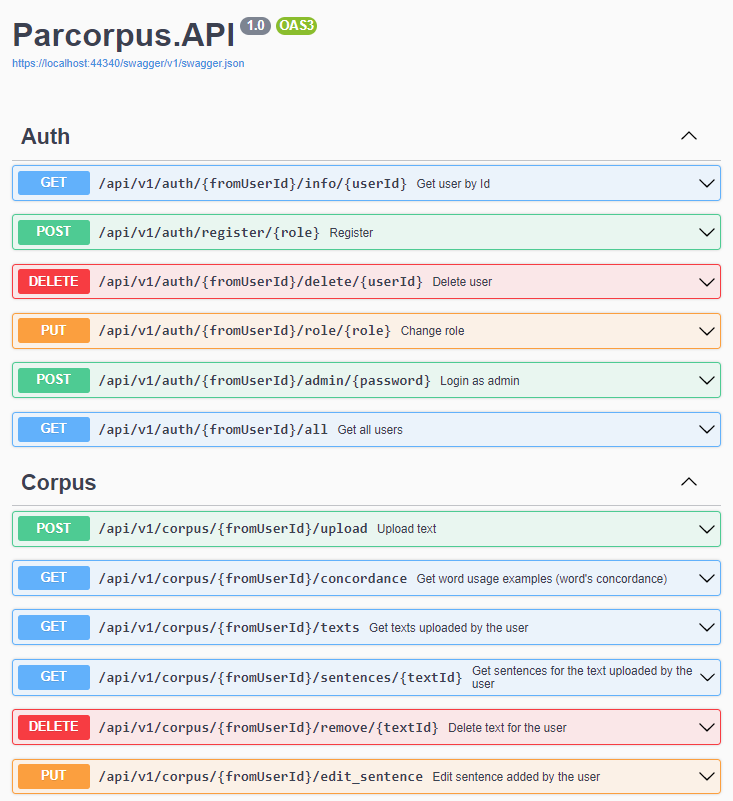
\includegraphics[scale=1]{img/swagger}
	\caption{Swagger UI}
	\label{swagger}
\end{figure}

\clearpage

Чтобы сделать какое-либо действие, необходимо выбрать секцию с необходимой конечной точкой и ввести необходимые данные. 
Пример регистрации пользователя представлен на рисунке~\ref{register}.

\captionsetup{singlelinecheck = false, justification=centering}
\begin{figure}[ht]
	\centering
	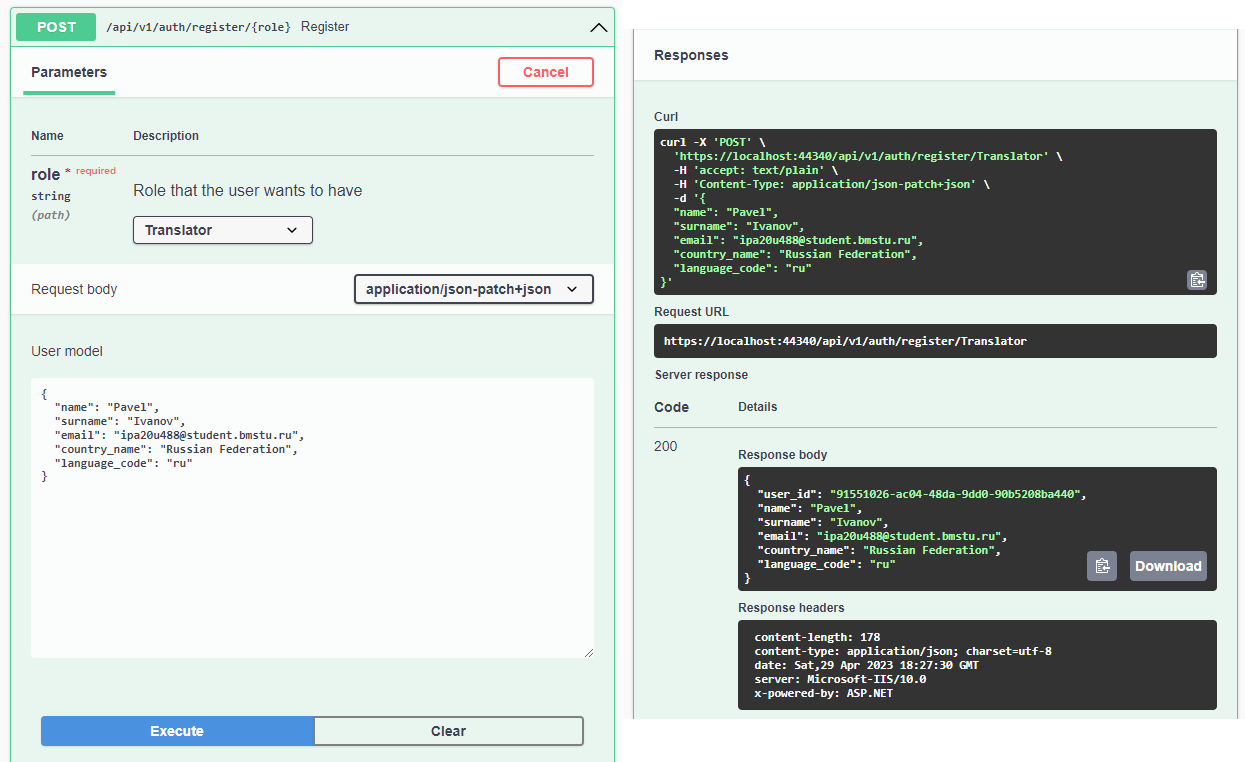
\includegraphics[width=\textwidth]{img/register}
	\caption{Пример регистрации пользователя}
	\label{register}
\end{figure}

Пример получения примеров употребления слова <<и>> на английском языке представлен на рисунке~\ref{concordance}. При данном запросе прочие фильтры отсутствуют, поэтому некоторым поля результата присвоено значение null.

\captionsetup{singlelinecheck = false, justification=centering}
\begin{figure}[H]
	\centering
	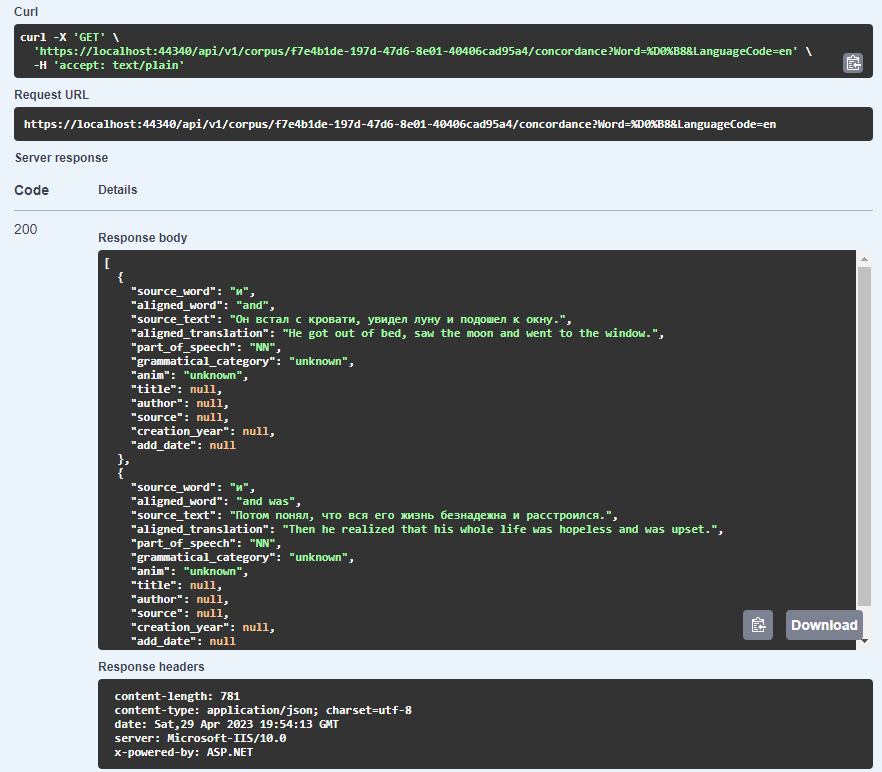
\includegraphics[width=\textwidth]{img/example}
	\caption{Пример получения примеров употребления слова}
	\label{concordance}
\end{figure}

\subsection{Логирование действий пользователей}

Для логирования действий пользователей используется платформа\\ NLog~--~бесплатный фреймворк для журналирования, совместимый со стеком ELK (Elasticsearch, Logstash, Kibana)~\cite{nlog}. Таким образом, генерируемые логи можно использовать в поисковых и аналитических движках. Фрагмент файла конфигурации представлен в листинге~\ref{nlog}.\\

\captionsetup{singlelinecheck = false, justification=raggedright}
\begin{lstlisting}[caption={Фрагмент файла NLog.config}, label=nlog]
<target name="asyncAllfile"
	    xsi:type="AsyncWrapper"
		timeToSleepBetweenBatches="0"
		overflowAction="Discard"
		batchSize="300" >
	<!-- write logs to file  -->
	<target name="allfile"
			xsi:type="File"
			encoding="utf-8"
			fileName="\${basedir}/log/\${shortdate}.log"
			layout="\${longdate}|\${var:logId}\${guid}|
					\${level:uppercase=true}|\${var:machineName}|
					\${message}|
					\${exception:maxInnerExceptionLevel=7}|
					\${callsite}"
			archiveFileName="\${basedir}/log/archives/{#}.log"
			archiveEvery="Day"
			archiveNumbering="Date"
			archiveDateFormat="yyyy-MM-dd"
			concurrentWrites="true"/>
</target>
\end{lstlisting}

Логи сохраняются в txt файлах в папке log с именем, соответствующем текущей дате в формате <<yyy-MM-dd>>. 
Автоматическое архивирование логов происходит каждый день. Формат записи сообщения в журнале предусматривает запись о дате, уникальном идентификаторе лога, уровне логирования, названии сервера, исключении (с максимальным уровнем вложенности 7) и компоненте, в котором происходит журналирование.

Пример сообщений в журнале при регистрации пользователя представлен в листинге~\ref{reg-log}.\\

\captionsetup{singlelinecheck = false, justification=raggedright}
\begin{lstlisting}[caption={Фрагмент логов при регистрации пользователя}, label=reg-log]
2023-04-30 11:37:40.7594|LogId:cf0cc6a99e144680a79cf6727e9c7054|
INFO|Server|Request starting HTTP/2 POST 
https://localhost:44340/api/v1/auth/register/Translator application/json-patch+json 150||
Microsoft.AspNetCore.Hosting.HostingApplicationDiagnostics.LogRe- questStarting
...
2023-04-30 11:37:44.5283|LogId:0417512af22c409586a443f95579b39e|
INFO|Server|Executed DbCommand (72ms) [Parameters=[@__countryName_0='?'], CommandType='Text', CommandTimeout='30']
SELECT c.country_id, c.name
FROM parcorpusdb.country AS c
WHERE c.name = @__countryName_0
LIMIT 1||Microsoft.EntityFrameworkCore.Diagnostics
.EventDefinition`6.Log

2023-04-30 11:37:44.6832|LogId:6c5d01f84b954671ad9ac7e057cbed29|
INFO|Server|Executed DbCommand (8ms) [Parameters=[@__languageShortName_0='?'], CommandType='Text', CommandTimeout='30']
SELECT l.language_id, l.full_name, l.short_name
FROM parcorpusdb.language AS l
WHERE l.short_name = @__languageShortName_0
LIMIT 1||
Microsoft.EntityFrameworkCore.Diagnostics
.EventDefinition`6.Log

2023-04-30 11:37:45.1292|LogId:37342430a3fa4fdc9bc2fc05177f4ed9|
INFO|Server|Executed DbCommand (55ms) [Parameters=[@p0='?' (DbType = Guid), @p1='?' (DbType = Int32), @p2='?', @p3='?', @p4='?' (DbType = Int32), @p5='?'], CommandType='Text', CommandTimeout='30']
\end{lstlisting}

\begin{lstlisting}[title={Окончание листинга \ref{reg-log}}, label=reg-log1, firstnumber=25]
INSERT INTO parcorpusdb."user" (user_id, country, email, name, native_language, surname)
VALUES (@p0, @p1, @p2, @p3, @p4, @p5);||
Microsoft.EntityFrameworkCore.Diagnostics.EventDefinition`6.Log

2023-04-30 11:37:53.2174|LogId:3ce6e47b6a504f49bc8e497ec696801c|
INFO|Server|Executed DbCommand (17ms) [Parameters=[], CommandType='Text', CommandTimeout='30']
create user "5182a73d-194a-4665-9651-a8c862571daf";||
Microsoft.EntityFrameworkCore.Diagnostics.EventDefinition`6.Log

2023-04-30 11:37:53.2891|LogId:a0aaf2140d264e06b72d430597aee1b2|
INFO|Server|Executed DbCommand (64ms) [Parameters=[], CommandType='Text', CommandTimeout='30']
grant translator to "5182a73d-194a-4665-9651-a8c862571daf";||
Microsoft.EntityFrameworkCore.Diagnostics.EventDefinition`6.Log
...
2023-04-30 11:37:53.4192|LogId:221418d9b0ba4538b118b2fd5d90a091|
INFO|Server|Request finished HTTP/2 POST https://localhost:44340/api/v1/auth/register/Translator application/json-patch+json 150 - 200 178 application/json;+charset=utf-8 12663.1748ms||
Microsoft.AspNetCore.Hosting.HostingApplicationDiagnostics
.LogRequestFinished
\end{lstlisting}

\subsection{Инструкция для развертывания системы}

Для развертывания разработанной системы необходимо установить \\Docker~--~программное обеспечение для автоматизации развертывания и управления приложениями в средах с поддержкой контейнеризации~\cite{docker}. 
Docker доступен как на Windows, так и на Linux или MacOS. 

Для запуска системы на компьютере или на сервере необходимо проделать следующие действия:

\begin{enumerate}
	\item открыть терминал в директории приложения (в ней находятся папки doc, src и test);
	
	\item ввести команду <<cd ./src/Scripts \&\& docker-compose up -d>>.
\end{enumerate}

После нажатия Enter система Docker самостоятельно скачает и установит все необходимые пакеты, а также запустит СУБД и сервисы приложения. 
Пример вывода консоли при запуске системы представлен в листинге~\ref{docker-ex}.

\captionsetup{singlelinecheck = false, justification=raggedright}
\begin{lstlisting}[caption={Запуск системы}, label=docker-ex]
C:\Users\Pavel\Desktop\parcorpus\src\Scripts>
docker-compose up -d
[+] Running 5/5
Network scripts_backend-network Created 0.1s
Container redis                 Started 3.0s
Container aligner               Started 3.2s
Container postgres              Started 3.4s
Container parcorpus-backend     Started
\end{lstlisting}

После запуска системы её записи журнала доступны на локальной машине и находятся в папке /src/Parcorpus/Parcorpus.API/logs. Изменение настроек (например, строки подключения к базе данных или кеширующей СУБД) доступно в файле /src/Parcorpus/Parcorpus.API/appsettings.json. При изменении данного файла будет также изменен файл в контейнере.

После запуска системы взаимодействие может с ней осуществляется по адресу http://localhost:802/. Список доступных конечных точек соединения по данному адресу представлен в таблице~\ref{endpoints}.

\begin{table}[H]\caption{Конечные точки соединения}\label{endpoints}
	\begin{tabular}{|l|l|l|}
		\hline
		\multicolumn{1}{|c|}{Конечная точка} &
		\multicolumn{1}{c|}{Параметры} &
		\multicolumn{1}{c|}{Описание} \\ \hline
		\begin{tabular}[c]{@{}l@{}}GET: /api/v1/auth/\\ \{fromUserId\}/info/\\ \{userId\}\end{tabular} &
		\begin{tabular}[c]{@{}l@{}}fromUserId -- идентификатор \\ пользователя, который \\ совершает запрос;\\ userId -- идентификатор \\ пользователя, о \\ котором запрашивается \\ информация.\end{tabular} &
		\begin{tabular}[c]{@{}l@{}}Получение \\ информации \\ о пользователе\end{tabular} \\ \hline
		\begin{tabular}[c]{@{}l@{}}DELETE: /api/v1/auth/\\ \{fromUserId\}/delete/\\\{userId\}\end{tabular} &
		\begin{tabular}[c]{@{}l@{}}fromUserId -- идентификатор \\ пользователя, \\ который совершает \\ запрос;\\ userId -- идентификатор \\ удаляемого \\ пользователя.\end{tabular} &
		\begin{tabular}[c]{@{}l@{}}Удаление \\ пользователя\end{tabular} \\ \hline
		\begin{tabular}[c]{@{}l@{}}PUT: /api/v1/auth/\\ \{fromUserId\}/role/\{role\}\end{tabular} &
		\begin{tabular}[c]{@{}l@{}}fromUserId -- идентификатор \\ пользователя, \\ который совершает запрос;\\ role -- новая роль пользователя.\end{tabular} &
		Смена роли \\ \hline
		\begin{tabular}[c]{@{}l@{}}POST: \\/api/v1/auth/register/\{role\}\end{tabular} &
		\begin{tabular}[c]{@{}l@{}}role -- роль регистрируемого \\ пользователя;\\ Тело запроса \\ (application/json-patch+json): \\ UserRegistrationDto.\end{tabular} &
		\begin{tabular}[c]{@{}l@{}}Регистрация \\ нового \\ пользователя\end{tabular} \\ \hline
	\end{tabular}
\end{table}

\begin{table}[H]\caption*{Продолжение таблицы~\ref{endpoints}}
	\begin{tabular}{|l|l|l|}
		\hline
		\multicolumn{1}{|c|}{Конечная точка} &
		\multicolumn{1}{c|}{Параметры} &
		\multicolumn{1}{c|}{Описание} \\ \hline
		\begin{tabular}[c]{@{}l@{}}POST:\\/api/v1/auth/\\ \{fromUserId\}/admin/\\ \{password\}\end{tabular} &
		\begin{tabular}[c]{@{}l@{}}fromUserId -- идентификатор \\ пользователя, \\ который совершает запрос;\\ password -- пароль.\end{tabular} &
		\begin{tabular}[c]{@{}l@{}}Авторизация \\ администратора\end{tabular} \\ \hline
		\begin{tabular}[c]{@{}l@{}}GET: \\/api/v1/auth/\\ \{fromUserId\}/all\end{tabular} &
		\begin{tabular}[c]{@{}l@{}}fromUserId -- идентификатор \\ пользователя, \\ который совершает запрос.\end{tabular} &
		\begin{tabular}[c]{@{}l@{}}Получение \\ информации о всех \\ пользователях\end{tabular} \\ \hline
		\begin{tabular}[c]{@{}l@{}}POST:\\/api/v1/corpus/\\ \{fromUserId\}/upload\end{tabular} &
		\begin{tabular}[c]{@{}l@{}}fromUserId -- идентификатор \\ пользователя, \\ который совершает запрос.\\ Тело запроса \\ (multipart/form-data): \\ InputTextDto.\end{tabular} &
		\begin{tabular}[c]{@{}l@{}}Загрузка нового текста\end{tabular} \\ \hline
		\begin{tabular}[c]{@{}l@{}}GET:\\/api/v1/corpus/\\ \{fromUserId\}/\\ concordance\end{tabular} &
		\begin{tabular}[c]{@{}l@{}}fromUserId -- идентификатор \\ пользователя, \\ который совершает запрос.\\ Тело запроса \\ (multipart/form-data): \\ ConcordanceQueryDto.\end{tabular} &
		\begin{tabular}[c]{@{}l@{}}Поиск примеров \\ употребления \\ слова\end{tabular} \\ \hline
		\begin{tabular}[c]{@{}l@{}}GET:\\/api/v1/corpus/\\ \{fromUserId\}/texts\end{tabular} &
		\begin{tabular}[c]{@{}l@{}}fromUserId -- идентификатор \\ пользователя, \\ который совершает запрос;\end{tabular} &
		\begin{tabular}[c]{@{}l@{}}Получение всех \\ текстов \\ пользователя\end{tabular} \\ \hline
	\end{tabular}
\end{table}

\begin{table}[H]\caption*{Окончание таблицы~\ref{endpoints}}
	\begin{tabular}{|l|l|l|}
		\hline
		\multicolumn{1}{|c|}{Конечная точка} &
		\multicolumn{1}{c|}{Параметры} &
		\multicolumn{1}{c|}{Описание} \\ \hline
		\begin{tabular}[c]{@{}l@{}}GET:\\/api/v1/corpus/\\ \{fromUserId\}/sentences/\\ \{textId\}\end{tabular} &
		\begin{tabular}[c]{@{}l@{}}fromUserId -- идентификатор \\ пользователя, \\ который совершает запрос;\\ textId -- идентификатор текста.\end{tabular} &
		\begin{tabular}[c]{@{}l@{}}Получение всех \\ предложений \\ добавленного \\ пользователем \\ текста\end{tabular} \\ \hline
		\begin{tabular}[c]{@{}l@{}}DELETE:\\/api/v1/corpus/\\ \{fromUserId\}/remove/\\ \{textId\}\end{tabular} &
		\begin{tabular}[c]{@{}l@{}}fromUserId -- идентификатор \\ пользователя, \\ который совершает запрос;\\ textId -- идентификатор текста.\end{tabular} &
		Удаление текста \\ \hline
		\begin{tabular}[c]{@{}l@{}}PUT:\\/api/v1/corpus/\\ \{fromUserId\}/\\ edit\_sentence\end{tabular} &
		\begin{tabular}[c]{@{}l@{}}fromUserId -- идентификатор \\ пользователя, \\ который совершает запрос;\\ Тело запроса \\ (application/json-patch+json): \\ SentenceDto.\end{tabular} &
		\begin{tabular}[c]{@{}l@{}}Редактирование \\ предложения\end{tabular} \\ \hline
	\end{tabular}
\end{table}

Упомянутые объекты передачи данных (англ. <<Data transfer object>>,\\ <<DTO>>) имеют структуру, представленную в листингах~\ref{dto1}--\ref{dto5}.

\captionsetup{singlelinecheck = false, justification=raggedright}
\begin{lstlisting}[caption={UserRegistrationDto}, language=c++, label=dto1]
public class UserRegistrationDto
{
	/// <summary>  §Имя пользователя§  </summary>
	/// <example>Pavel</example>
	[JsonProperty("name")]
	public string Name { get; set; }
	
	/// <summary> §Фамилия пользователя§ </summary>
\end{lstlisting}

\begin{lstlisting}[title={Окончание листинга \ref{dto1}}, language=c++, label=dto11, firstnumber=9]
	/// <example>Ivanov</example>
	[JsonProperty("surname")]
	public string Surname { get; set; }
	
	/// <summary> §Электронная почта пользователя§ </summary>
	/// <example>ipa20u488@student.bmstu.ru</example>
	[JsonProperty("email")]
	public string Email { get; set; }
	
	/// <summary> §Название страны пользователя§ </summary>
	/// <example>Russian Federation</example>
	[JsonProperty("country_name")]
	public string CountryName { get; set; }
	
	/// <summary>
	/// §Сокращенное название родного языка пользователя§
	/// </summary>
	/// <example>ru</example>
	[JsonProperty("language_code")]
	public string LanguageCode { get; set; }
}
\end{lstlisting}

\begin{lstlisting}[caption={InputTextDto}, language=c++, label=dto2]
public class InputTextDto
{
	/// <summary> §Сокращенное название исходного языка§ </summary>
	/// <example>ru</example>
	public string SourceLanguageCode { get; set; }
	
	/// <summary> §Сокращенное название целевого языка§ </summary>
	/// <example>en</example>
	public string TargetLanguageCode { get; set; }
\end{lstlisting}

\begin{lstlisting}[title={Окончание листинга \ref{dto2}}, language=c++, label=dto21, firstnumber=10]	
	/// <summary> §Название текста§ </summary>
	public string? Title { get; set; }
	
	/// <summary> §Автор текста§ </summary>
	public string? Author { get; set; }
	
	/// <summary> §Источник текста§ </summary>
	public string? Source { get; set; }
	
	/// <summary> §Год написания текста§ </summary>
	public int? CreationYear { get; set; }
	
	/// <summary> §Перечисление жанров§ </summary>
	public IEnumerable<string> Genres { get; set; }
	
	/// <summary> §Файл с исходным текстом§ </summary>
	[FromForm(Name="SourceText")]
	public IFormFile SourceText { get; set; }
	
	/// <summary> §Файл с переведенным текстом§ </summary>
	[FromForm(Name="TargetText")]
	public IFormFile TargetText { get; set; }
}
\end{lstlisting}

\begin{lstlisting}[caption={ConcordanceQueryDto}, language=c++, label=dto3]
public class ConcordanceQueryDto
{
	/// <summary> §Слово для поиска§ </summary>
	[JsonProperty("word")]
	public string Word { get; set; }
	
	/// <summary> §Краткое название целевого языка§ </summary>
\end{lstlisting}

\begin{lstlisting}[title={Окончание листинга \ref{dto3}}, language=c++, label=dto31, , firstnumber=8]
	/// <example>"ru"</example>
	[JsonProperty("language_code")]
	public string LanguageCode { get; set; }
	
	/// <summary> §Фильтры поиска§ </summary>
	[JsonProperty("filter")]
	public FilterDto? Filter { get; set; }
}
\end{lstlisting}

\begin{lstlisting}[caption={FilterQueryDto}, language=c++, label=dto4]
public class FilterDto
{
	/// <summary> §Жанр§ </summary>
	[JsonProperty("genre")]
	public string? Genre { get; set; }
	
	/// <summary> §Дата начала§ </summary>
	[JsonProperty("start_date_time")]
	public DateTime? StartDateTime { get; set; }
	
	/// <summary> §Дата окончания§ </summary>
	[JsonProperty("end_date_time")]
	public DateTime? EndDateTime { get; set; }
	
	/// <summary> §Часть речи§ </summary>
	[JsonProperty("part_of_speech")]
	public string? Pos { get; set; }
	
	/// <summary> §Грамматическая категория§ </summary>
	[JsonProperty("gram")]
	public string? Gram { get; set; }
	
	/// <summary> §Одушевленность§ </summary>
\end{lstlisting}

\begin{lstlisting}[title={Окончание листинга \ref{dto4}}, language=c++, label=dto41, firstnumber=24]
	[JsonProperty("anim")]
	public string? Anim { get; set; }
	
	/// <summary> §Автор§ </summary>
	[JsonProperty("author")]
	public string? Author { get; set; }
}
\end{lstlisting}

\begin{lstlisting}[caption={SentenceDto}, language=c++, label=dto5]
public class SentenceDto
{
	/// <summary> §Id предложения§ </summary>
	[JsonProperty("sentence_id")]
	public int? SentenceId { get; set; }
	
	/// <summary> 
	/// §Новый текст предложения на исходном языке§ 
	/// </summary>
	/// <example>I saw an apple</example>
	[JsonProperty("source_text")]
	public string? SourceText { get; set; }
	
	/// <summary> §Новый перевод§ </summary>
	/// <example>§Я увидел яблоко§</example>
	[JsonProperty("aligned_translation")]
	public string? AlignedTranslation { get; set; }
}
\end{lstlisting}
\newpage
Общая последовательность действий при работе с системой следующая:
\begin{enumerate}
	\item Регистрация и получение UserId.
	\begin{lstlisting}
curl -X 'POST' \
	'http://localhost:802/api/v1/auth/register/Translator' \
	-H 'accept: text/plain' \
	-H 'Content-Type: application/json-patch+json' \
	-d '{ \
		"name": "Peter", \
		"surname": "Parker", \
		"email": "ipa20u488@student.bmstu.ru", \
		"country_name": "Russian Federation", \
		"language_code": "ru" \
	}'
\end{lstlisting}
	В качестве ответа возвращается JSON, содержащий UserId.
	\begin{lstlisting}
{
	"user_id": "9c95e47a-9617-4ab3-b80d-b31055a97f19",
	"name": "Peter",
	"surname": "Parker",
	"email": "ipa20u488@student.bmstu.ru",
	"country_name": "Russian Federation",
	"language_code": "ru"
}
	\end{lstlisting}

	\item Запомнив UserId, можно выполнять любые запросы. Например, получение примеров употребления.
	\begin{lstlisting}
curl -X 'GET' \
	'http://localhost:802/api/v1/corpus/ \
	9c95e47a-9617-4ab3-b80d-b31055a97f19/concordance? \
	Word=%D0%B8&LanguageCode=en&Filter.Genre=Drama' \
	-H 'accept: text/plain'
	\end{lstlisting}
\pagebreak
Полученный ответ:
	\begin{lstlisting}
[
	{
		"source_word": §"и"§,
		"aligned_word": "and",
		"source_text": §"Он встал с кровати, увидел луну и §
						§ подошел к окну."§,
		"aligned_translation": "He got out of bed, saw the 
							moon and went to the window.",
		"part_of_speech": "NN",
		"grammatical_category": "unknown",
		"anim": "unknown",
		"title": "My example 1",
		"author": "Pavel Ivanov",
		"source": "Pavel Ivanov",
		"creation_year": "2023-01-01",
		"add_date": "2023-04-29"
	}, {
		"source_word": §"и"§,
		"aligned_word": "and was",
		"source_text": §"Потом понял, что вся его жизнь §
						§безнадежна и расстроился."§,
		"aligned_translation": "Then he realized that his 
				  whole life was hopeless and was upset.",
		"part_of_speech": "NN",
		"grammatical_category": "unknown",
		"anim": "unknown",
		"title": "My example 1",
		"author": "Pavel Ivanov",
		"source": "Pavel Ivanov",
		"creation_year": "2023-01-01",
		"add_date": "2023-04-29"
	}
]
	\end{lstlisting}

	\item Возможна аутентификация в качестве администратора. Для этого необходимо ввести пароль: pavelivanovIU7-65B.
	
	\begin{lstlisting}
curl -X 'POST' \
	'http://localhost:802/api/v1/auth/ \
		9c95e47a-9617-4ab3-b80d-b31055a97f19/admin/ \
		pavelivanovIU7-65B' \
	-H 'accept: */*' \
	-d ''
	\end{lstlisting}

	В случае успеха возвращается код 200.
\end{enumerate}

\subsection{Тестирование}

В результате тестирования ролей получены результаты, представленные в таблице~\ref{roles-table}. 
Как видно из полученных результатов, разработанная система соответствует спроектированной ролевой модели. 
В случае отсутствия прав возвращается ошибка 401. В методах sentences, remove и edit\_sentence ошибка 401 возникает в случае обращения к тексту, который добавил другой пользователь (кроме случая администратора).

\begin{table}[H]\caption{Результаты тестирования разделения ролей}\label{roles-table}
	\begin{tabular}{|l|l|l|}
		\hline
		\multicolumn{1}{|c|}{Роль} & \multicolumn{1}{c|}{Конечная точка}                                                           & \multicolumn{1}{c|}{Ответ} \\ \hline
		Translator | Admin         & \begin{tabular}[c]{@{}l@{}}/api/v1/corpus/\{fromUserId\}/\\ upload\end{tabular}               & 201 / 409                  \\ \hline
		Teacher                    & \begin{tabular}[c]{@{}l@{}}/api/v1/corpus/\{fromUserId\}/\\ upload\end{tabular}               & 401                        \\ \hline
		Teacher | Translator | Admin    & \begin{tabular}[c]{@{}l@{}}/api/v1/corpus/\{fromUserId\}/\\ concordance\end{tabular}          & 200 / 404       \\ \hline
		Translator | Translator | Admin & \begin{tabular}[c]{@{}l@{}}/api/v1/corpus/\{fromUserId\}/\\ texts\end{tabular}                & 200 / 404       \\ \hline
		Translator | Teacher            & \begin{tabular}[c]{@{}l@{}}/api/v1/corpus/\{fromUserId\}/\\ sentences/\{textId\}\end{tabular} & 200 / 401 / 404 \\ \hline
		Admin                      & \begin{tabular}[c]{@{}l@{}}/api/v1/corpus/\{fromUserId\}/\\ sentences/\{textId\}\end{tabular} & 200 / 404                  \\ \hline
		Translator | Teacher            & \begin{tabular}[c]{@{}l@{}}/api/v1/corpus/\{fromUserId\}/\\ remove/\{textId\}\end{tabular}    & 200 / 401 / 404 \\ \hline
		Admin                      & \begin{tabular}[c]{@{}l@{}}/api/v1/corpus/\{fromUserId\}/\\ remove/\{textId\}\end{tabular}    & 200 / 404                  \\ \hline
		Translator | Teacher            & \begin{tabular}[c]{@{}l@{}}/api/v1/corpus/\{fromUserId\}/\\ edit\_sentence\end{tabular}       & 200 / 401 / 404 \\ \hline
		Admin                      & \begin{tabular}[c]{@{}l@{}}/api/v1/corpus/\{fromUserId\}/\\ edit\_sentence\end{tabular}       & 200 / 404                  \\ \hline
		Translator | Teacher       & \begin{tabular}[c]{@{}l@{}}/api/v1/auth/\{fromUserId\}/\\ info/\{userId\}\end{tabular}        & 401                        \\ \hline
		Admin                      & \begin{tabular}[c]{@{}l@{}}/api/v1/auth/\{fromUserId\}/\\ info/\{userId\}\end{tabular}        & 200 / 404                  \\ \hline
	\end{tabular}
\end{table}

\begin{table}[H]\caption*{Окончание таблицы~\ref{roles-table}}
	\begin{tabular}{|l|l|l|}
		\hline
		\multicolumn{1}{|c|}{Роль} & \multicolumn{1}{c|}{Конечная точка}                                                           & \multicolumn{1}{c|}{Ответ} \\ \hline
		Translator | Teacher            & \begin{tabular}[c]{@{}l@{}}/api/v1/auth/\{fromUserId\}/\\ delete/\{userId\}\end{tabular}      & 401             \\ \hline
		Admin                      & \begin{tabular}[c]{@{}l@{}}/api/v1/auth/\{fromUserId\}/\\ delete/\{userId\}\end{tabular}      & 200 / 404                  \\ \hline
		Translator | Teacher | Admin    & \begin{tabular}[c]{@{}l@{}}/api/v1/auth/\{fromUserId\}/\\ admin/\{password\}\end{tabular}     & 200 / 403       \\ \hline
		Translator | Teacher       & /api/v1/auth/\{fromUserId\}/all                                                               & 401                        \\ \hline
		Admin                      & /api/v1/auth/\{fromUserId\}/all                                                               & 200                        \\ \hline
	\end{tabular}
\end{table}

\subsection*{Вывод}

В данном разделе было приведено обоснование выбора средств реализации системы. 
В качестве основной реляционной СУБД была выбрана система с открытым кодом PostgreSQL, поскольку она является одной из самых быстрых (по операции чтения) СУБД. 
Для системы кеширования была выбрана In-Memory Database Redis, поскольку она является одной из самых быстрых NoSQL СУБД и предоставляет весь необходимый для решения поставленной задачи функционал.

Для написания интерфейса для взаимодействия с параллельным корпусом был выбран язык C$\#$, а для обработки лингвистических данных язык Python. 
В результате написано REST API на основе фреймворка ASP.NET Core, предоставляющее набор конечных точек для работы с корпусом. 
Разработанная система реализует спроектированную ролевую модель, систему журналирования действий пользователя и использование кеша для ускорения получения ответов на выборку данных из корпуса.
Тестирование разделения ролей показало, что разработанная система соответствует спроектированной ролевой модели.

\pagebreak